\documentclass{IEEEtran}

\usepackage[activate={true,nocompatibility},final,tracking=true,kerning=true,spacing=true,factor=1100,stretch=10,shrink=10]{microtype}
\linespread{1}

\usepackage{amsmath}
\usepackage{bm}
\usepackage{amssymb}
\usepackage{algorithm}
\usepackage{algorithmic}
\usepackage{stfloats}

\ifCLASSINFOpdf
   \usepackage[pdftex]{graphicx}
\else
   \usepackage[dvips]{graphicx}
\fi

\ifCLASSOPTIONcompsoc
  \usepackage[caption=false,font=normalsize,labelfont=sf,textfont=sf]{subfig}
\else
  \usepackage[caption=false,font=footnotesize]{subfig}
\fi

\usepackage[style=ieee,maxbibnames=1,minbibnames=1,maxcitenames=1,mincitenames=1,backend=biber,defernumbers=false]{biblatex}
\addbibresource{my_TOF_model.bib}

\begin{document}
\title{Impact of Axial Ring Splitting on Image Quality for the Cost Reduction of Total-Body PET}

\author{N.~Efthimiou~(\IEEEmembership{Member~IEEE}),
        A.C.~Whitehead~(\IEEEmembership{Student~Member~IEEE}),
        M.~Stockhoff~(\IEEEmembership{Student~Member~IEEE}), 
        C.~Thyssen~(\IEEEmembership{Student~Member~IEEE}),
        S.J.~Archibald
        and~S.~Vandenberghe~(\IEEEmembership{Senior~Member~IEEE})%
        
        \vspace{-0.5cm}
        
        \thanks{This project is supported by the European Cooperation for Science, Technology Action TD1401: Fast Advanced Scintillation Timing and Daisy Appeal Charity.}%
        \thanks{A.C.~Whitehead is supported by GE Healthcare.}%
        \thanks{N.~Efthimiou and S.J.~Archibald are with the PET research centre, Faculty of Health Sciences, University of Hull, Hull, HU6~7RX, UK (contact: \texttt{n.efthymiou@hull.ac.uk}).}%
        \thanks{A.C.~Whitehead is with the Institute of Nuclear Medicine, University College London, London, NW1~2BU, UK}%
        \thanks{M.~Stockhoff, C.~Thyssen  and S.~Vandenberghe are with Ghent University, Ghent, Belgium.}%
        \thanks{We thank Dr. A. Allam and his family for the generous donation to help found the PET Research Centre at the University of Hull and for their continued support.}}%

\maketitle
\vspace{-1cm}
    
\IEEEpeerreviewmaketitle
\vspace{-1cm}

\begin{abstract}
Total-Body PET (TB-PET) has high sensitivity, provides the means for simultaneous imaging of distant organs, offers fast kinetics using short-lived isotopes and paediatric applications. Recently, the first TB-PET scanner was presented and the first results were impressive. However, the cost of a TB-PET scanner is prohibiting. Therefore we propose a flexible detector configuration which will increase the axial field of view and keep the overall cost low. We propose axial ring splitting, which will separate the full rings into rings with only even or only odd numbered detectors. In performance investigation, three configurations were considered (a) full rings - low number of detectors, short Field-of-View (FOV) (b) split rings - low number of detectors, long FOV (c) full rings - high number of detectors, long FOV. It was shown that config. (c) demonstrated the highest prompt count rate, as expected. Config. (a) was marginally better than config. (b). The same trends were observed in terms of noise equivalent count rate. Images reconstructed with OSEM (12 susets, 72 it.) demonstrated the improved image quality and noise properties of the longer scanners over classic PET.

\end{abstract}

\vspace{-0.2cm}

\section{Introduction}
\IEEEPARstart{T}{otal-Body} PET (TB-PET) scanners are long axial Field-of-View (FOV) scanners, designed with the aim of imaging large portions of the body without bed movement~\cite{Cherry2018Total-BodyCare., Moskal2019FeasibilityTomograph}. The scientific interest in the novel imaging possibilities and technological challenges, has been surging. Finally, last year, the first commercial TB-PET scanner for human scanning was presented and the first scans reported~\cite{Leung2018PerformanceScanner, Badawi2019FirstScanner.}.

TB-PET scanners allow simultaneous imaging of distant organs, adding the possibility of investigating their mutual interactions. Other key areas include fast kinetics, injection of high activities of short-lived isotopes and the possibility of paediatric applications.

\begin{figure}
    \vspace{-0.2cm}
    
    \centering
    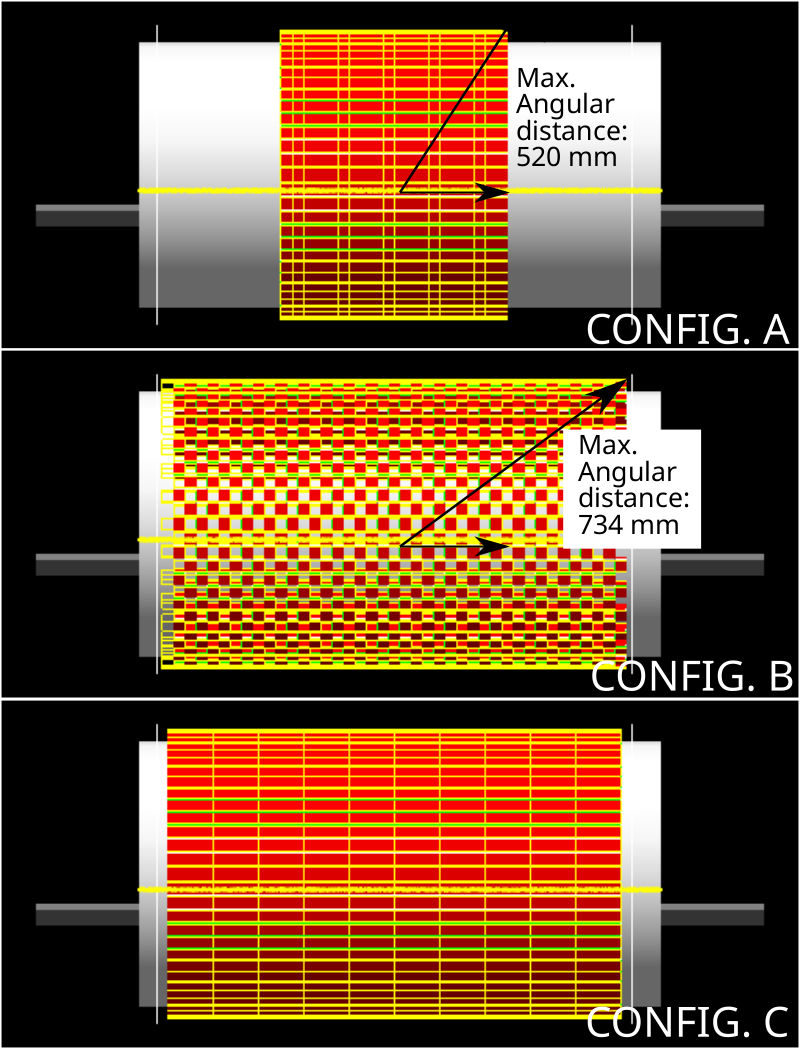
\includegraphics[width=0.85\linewidth]{dfd.png}
    \caption{The three configurations considered in this investigation. \textit{(The white cylinder is used for visualisation purposes)}}
    \label{fig:configs}
    
    \vspace{-0.2cm}
\end{figure}

The aim of this work is to try to find a more cost efficient way to build a TB-PET scanner.
In particular we investigated the possibility of a chess-like arrangement of detectors, by splitting each ring into a ring with the even detectors and a ring with the odd detectors (Fig.~\ref{fig:configs}). Hence, this will double the axial FOV while the number of detectors remains low. 

\vspace{-0.2cm}

\section{Methods}
The GATE~\cite{Jan2004} Monte Carlo toolkit was used for the simulation process. STIR~\cite{Thielemans2012P, Efthimiou2019ImplementationLibrary} was used for reconstruction and the processing of sinograms.

Three configurations were considered. A long axial FOV scanner with an axial length of $626$mm and a high number of detectors, a split ring configuration, where interchangeably rings lack either the odd or the even detectors, with an axial length of $1252$mm and a low number of detectors and finally a standard TB-PET scanner with full rings, axial length $1252$mm and a low number of detectors. The configurations were named: \texttt{Config.A}, \texttt{Config.B} and \texttt{Config.C}, respectively. The three configurations are illustrated in Fig~\ref{fig:configs}. 

Briefly, the system model is composed of blocks of $8 \times 8$ LYSO crystals with size $4 \times 4 \times 20$mm$^3$.  Each module either had one block (\texttt{Config.A}), a combination of block and gap (\texttt{Config.B}) or two blocks (\texttt{Config.B}).

The digitiser was the same as from a validated Philips Vereos scanner~\cite{Rausch2019PerformanceStandard} due to its high counting capabilities. 

Because the NEMA NU-2012~\cite{NationalElectricalManufacturersAssociation2012Performance2-2012} protocol is not optimised for such long scanners adaptations were made to the protocol. In particular the count losses phantom, which in the standard NEMA, has a length of $700$mm and was extended to $1500$mm, in order to provide a fair comparison between the long scanners and highlight the benefits of the longer axial FOV. In addition, the XCAT digital anthropomorphic phantom~\cite{Segars20104DResearch}, was also simulated.

\vspace{-0.2cm}

\section{Results}
\begin{figure}
    \vspace{-0.2cm}
    
    \centering
    \subfloat[\label{fig:prompts}]{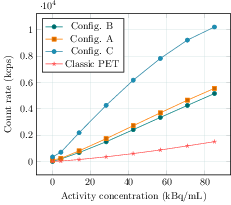
\includegraphics[width=0.5\linewidth]{allPrompts.png}}
    \subfloat[\label{fig:necr}]{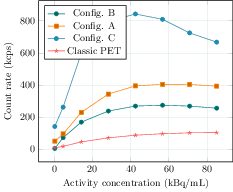
\includegraphics[width=0.5\linewidth]{allNECR.png}}
    \caption{(a) Prompt events (b) NECR for each configuration.}
    
    \vspace{-0.2cm}
\end{figure}

As can be seen in Fig.~\ref{fig:prompts}, in terms of detected prompts (trues + scattered + random) \texttt{Config.C} is far more efficient. \texttt{Config.C} was $\approx 8\%$ worse than \texttt{Config.A}, indicating that the axial expansion of the scanner does not compensate entirely for the introduction of the gaps. 

As illustrated in Fig.~\ref{fig:necr} in terms of Noise-Equivalent-Count-Rate(kcps) (NECR) \texttt{Config.C} is superior to the rest of configurations. However, its peak is located in one of the lower activity concentrations. Comparison between \texttt{Config.B} and \texttt{Config.A} showed that the NECR of \texttt{Config.A} is $25\%$ better, something that was not hinted at by the number of detected prompts. This shows that the true events lost, due to the gaps is proportionally more significant than for the scattered and random events, which are less affected.

\begin{figure}
    \vspace{-0.2cm}
    
    \centering
    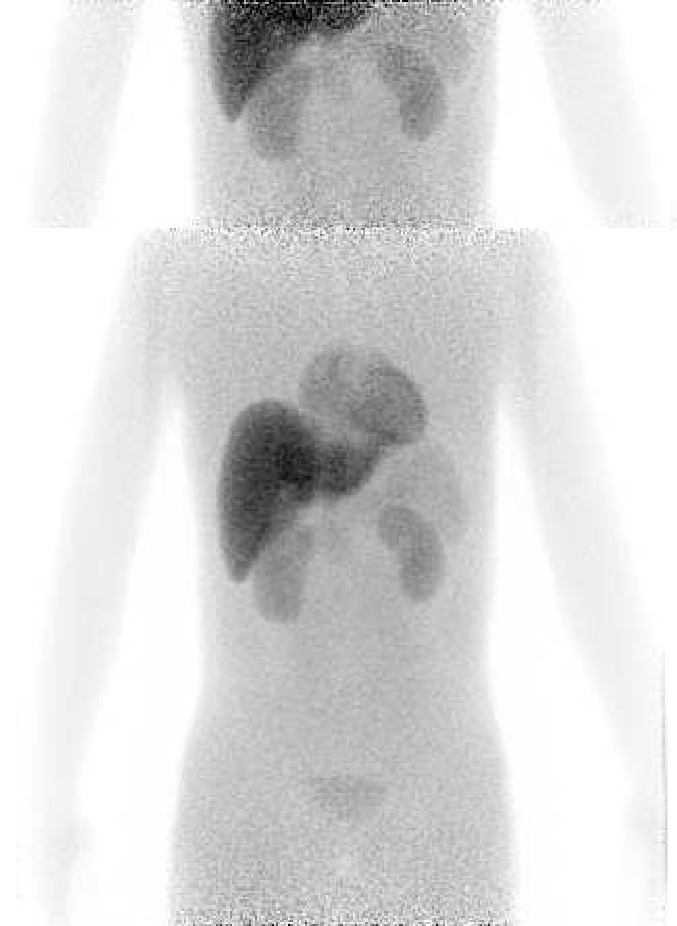
\includegraphics[width=0.85\linewidth]{recs.png}
    \caption{Images reconstructed with OSEM using $60$ iterations and $12$ subsets (a)classic PET scanner with a FOV of $240$mm and (b) \texttt{Config.A}. Applied corrections: normalisation, attenuation, scatter. Randoms were excluded.}
    \label{fig:recs}
    
    \vspace{-0.2cm}
\end{figure}

Moreover, the NECR of a PET scanner with a classic axial FOV of $240$mm, was included in order to highlight the benefits in sensitivity of the longer configurations. This is shown in Fig.~\ref{fig:recs} where images, reconstructed using OSEM with $60$ iterations and $12$ subsets, from the short scanner and from \texttt{Config.A} are demonstrated. The acquisition was that of a normal $^{18}$F-FDG biodistribution of $10$ seconds. In addition, to the wider FOV the longer scanner offers substantially better noise properties. 

\vspace{-0.2cm}

\section{Conclusion}
An alternative cost efficient design for a TB-PET scanner using a chess-like pattern of detectors, was evaluated in terms of count losses. This was compared to a compact configuration having the same number of detectors and a configuration with the same axial length and double the detectors. It was found that although the impact on the counting ability of the scanner is not significant the NECR is reduced by $25\%$. This hints that the detected true events suffer greater losses than the random and scattered. 

Currently our ability to reconstruct images of long PET scanner maxes out at $700$mm. In the future we plan to further extend this using more efficient memory management. 

\vspace{-0.2cm}
\AtNextBibliography{\footnotesize}
\printbibliography
\vspace{-0.2cm}

\end{document}
